
%(BEGIN_QUESTION)
% Copyright 2011, Tony R. Kuphaldt, released under the Creative Commons Attribution License (v 1.0)
% This means you may do almost anything with this work of mine, so long as you give me proper credit

Sketch the necessary connecting tubes (thick lines) and wires (thin lines) to make the fail-closed control valve {\it open wide} when the ``TRIP'' pushbutton is pressed.  Note that the solenoid valve requires 120 VAC, not 480 VAC:

$$\includegraphics[width=15.5cm]{i02213x01.eps}$$

\underbar{file i02213}
%(END_QUESTION)





%(BEGIN_ANSWER)

$$\includegraphics[width=15.5cm]{i02213x02.eps}$$

The tube coming off the top of the diaphragm should be left vented, as should the ``E'' port on the solenoid valve.  If the answer shows these two tubes connected together, deduct 5 points.

%(END_ANSWER)





%(BEGIN_NOTES)

{\bf This question is intended for exams only and not worksheets!}.

%(END_NOTES)


